\documentclass{beamer}

\usepackage{subcaption}
\usepackage{comment}
\usepackage{csvsimple, booktabs}


\usetheme{Warsaw}
\usecolortheme{wolverine}
\setbeamertemplate{headline}{} % not showing on top
%Information to be included in the title page:
\title{A simple detector for crowd counting using OpenCV and Python}
\author{Martí Gelabert Gómez}
\institute{University of the Balearic Islands}
\date{\today}

\begin{document}

\frame{\titlepage}

\frame{\tableofcontents}

\section*{Procedure}
\begin{frame}
\frametitle{Procedure}
\begin{enumerate}
    \item Import images as black and white.
    \item Apply Adaptative Histogram equalization to the images.
    \item Substract the background to the images using the image with the background.
    \item Apply an erosion algorithm to obtain small highlighted areas.
    \item Apply a thresholding algorithm to binarize the image.
    \item Apply a dilation operation into the binarized images to expand the whites.
    \item Use a contour algorithm to extract the diferent regions containing persons.
    \item Obtain the bounding boxes from these regions.
    \item Count them and compare the number of detections to the real cuantity.
\end{enumerate}\end{frame}


\section{Background Removal}
    \begin{frame}
        \frametitle{Background Removal}
        \begin{figure}
            \centering
            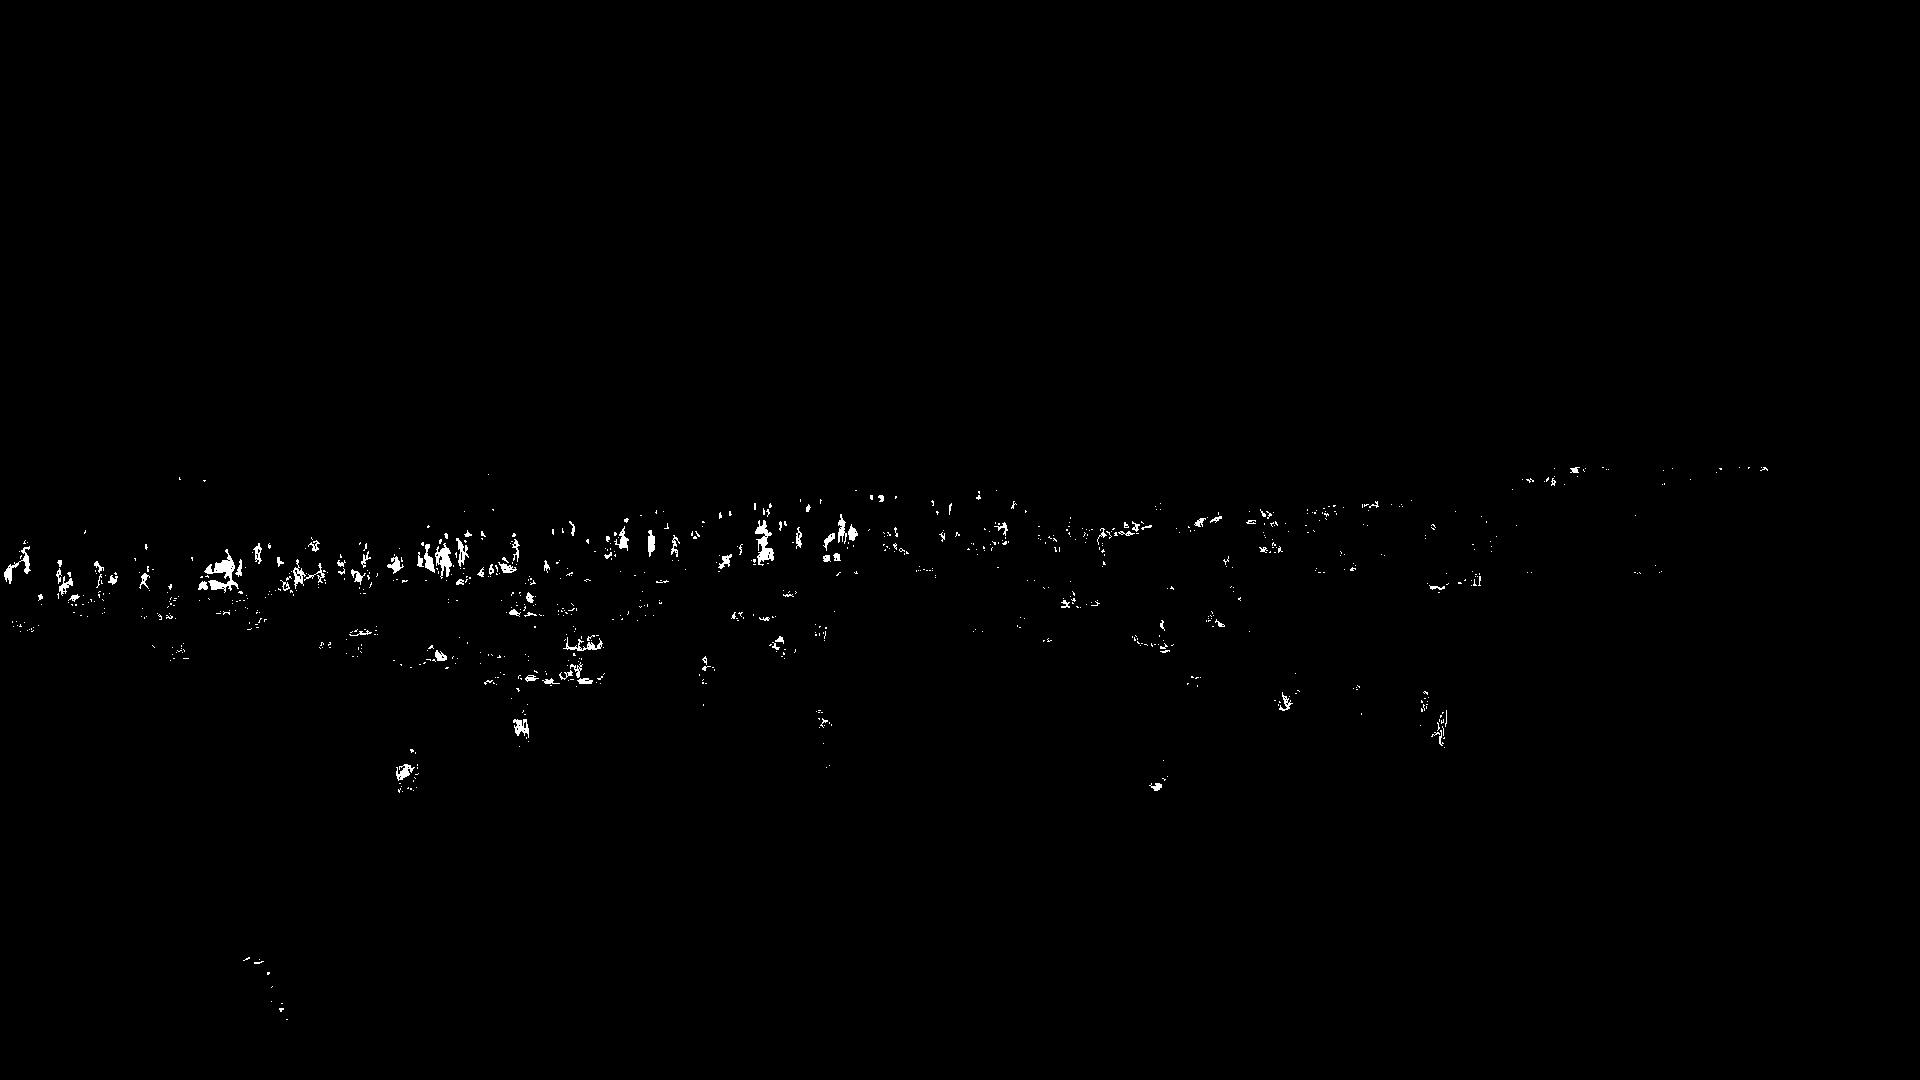
\includegraphics[width=\textwidth]{../gen/bin/1660320000.jpg}
        \end{figure}
    \end{frame}

\subsection*{CLAHE}
    \begin{frame}
        \frametitle{CLAHE}
        We need to do something with the mood of the images.
        \begin{columns}[c]
            % create the column with the first image, that occupies
            % half of the slide
                \begin{column}{.5\textwidth}
                \begin{figure}
                    \centering
                    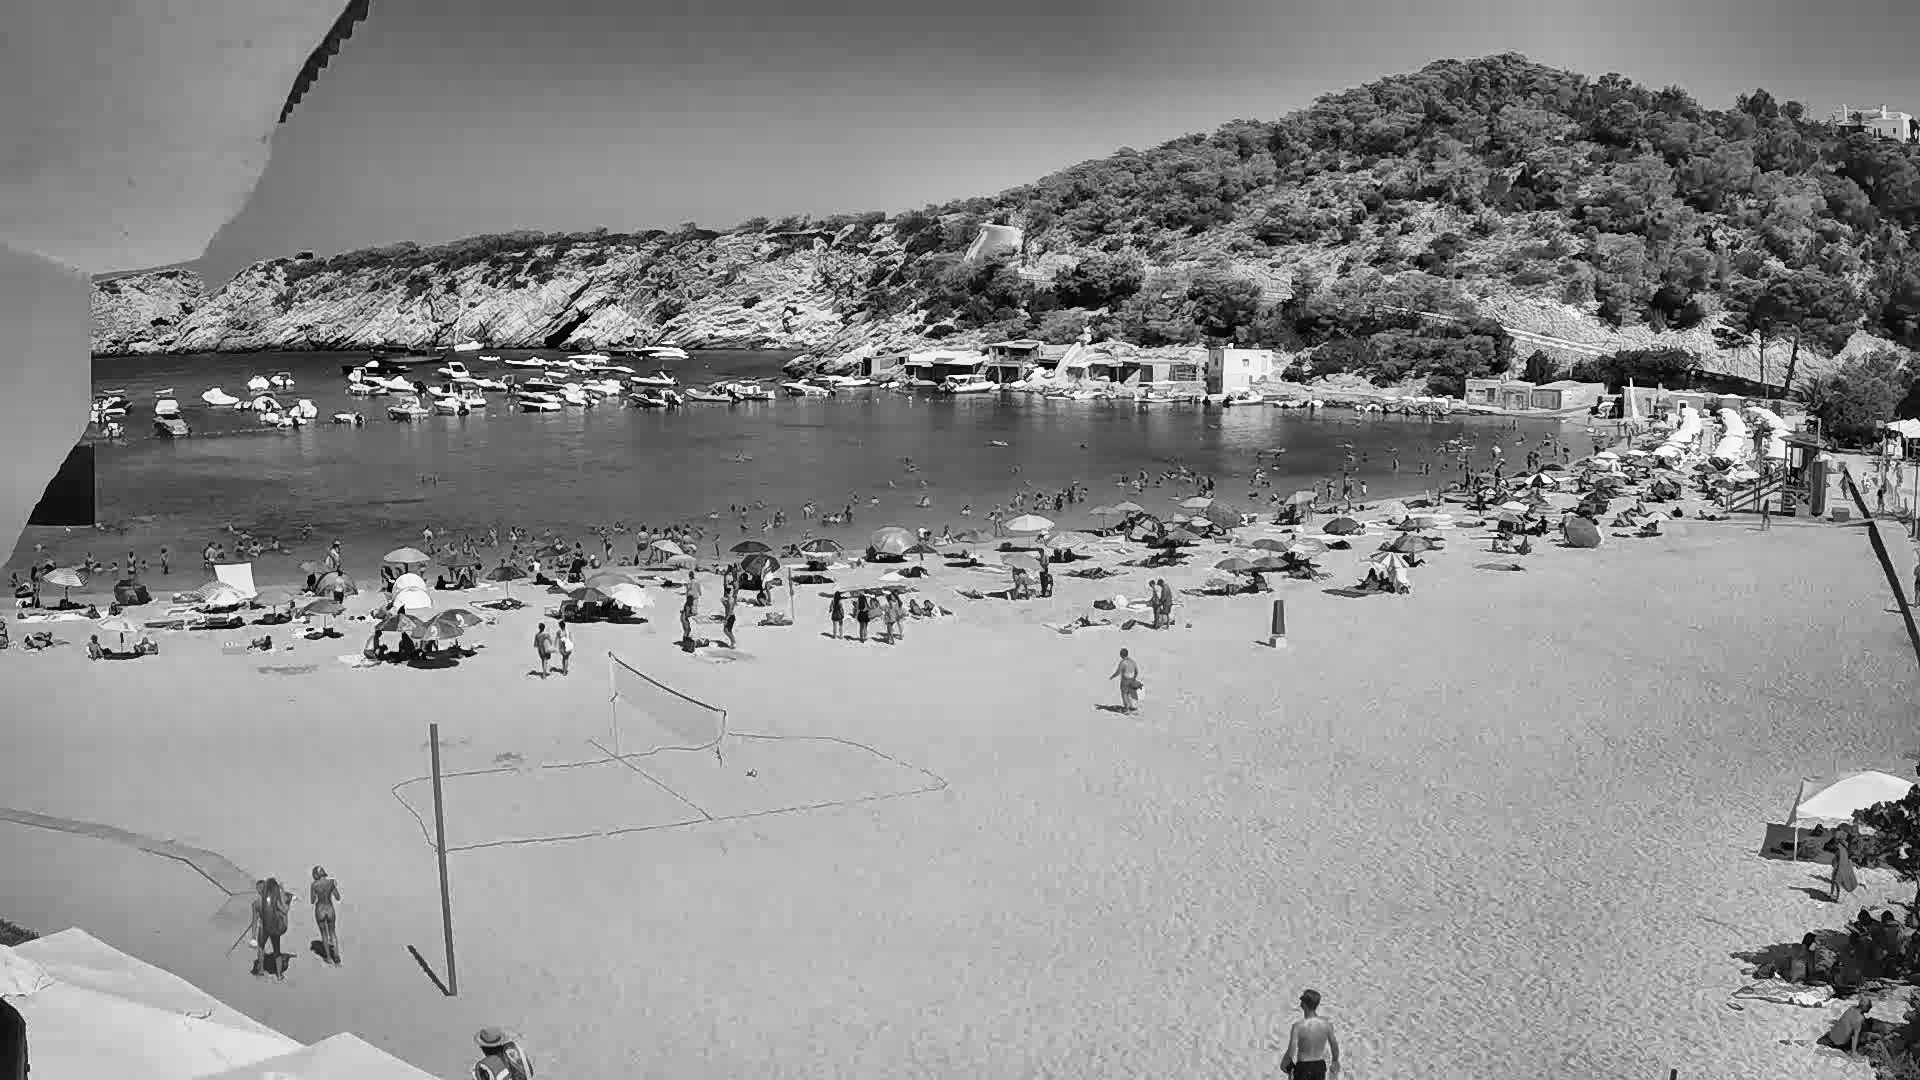
\includegraphics[width=\textwidth]{../gen/equ/1660298400.jpg}
                    
                \end{figure}      
                \end{column}
            % create the column with the second image, that also
            % occupies half of the slide
                \begin{column}{.5\textwidth}
                \begin{figure}
                    \centering
                    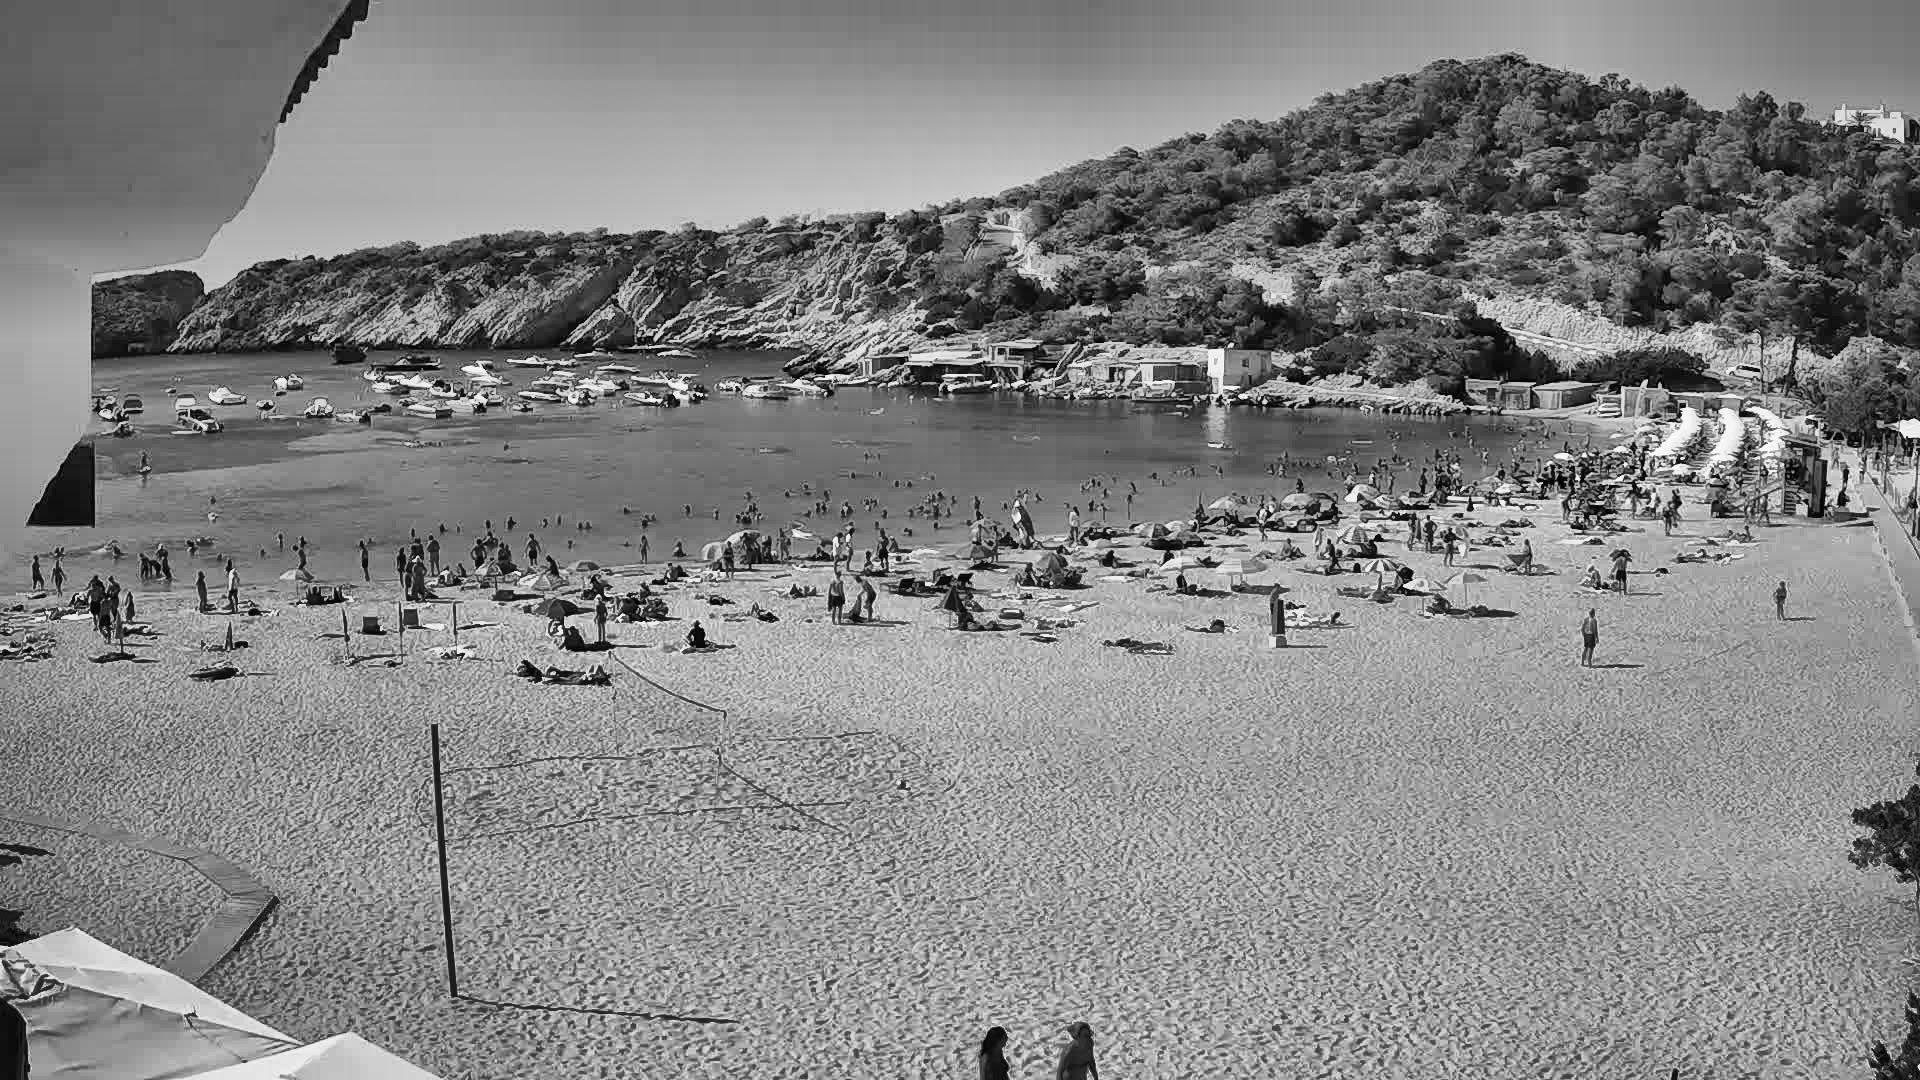
\includegraphics[width=\textwidth]{../gen/equ/1660316400.jpg}                 
                \end{figure}
                \end{column}
            \end{columns}

    \end{frame}

\subsection*{Background Image}
\begin{frame}
    \frametitle{Background Image}

    \begin{figure}
        \centering
        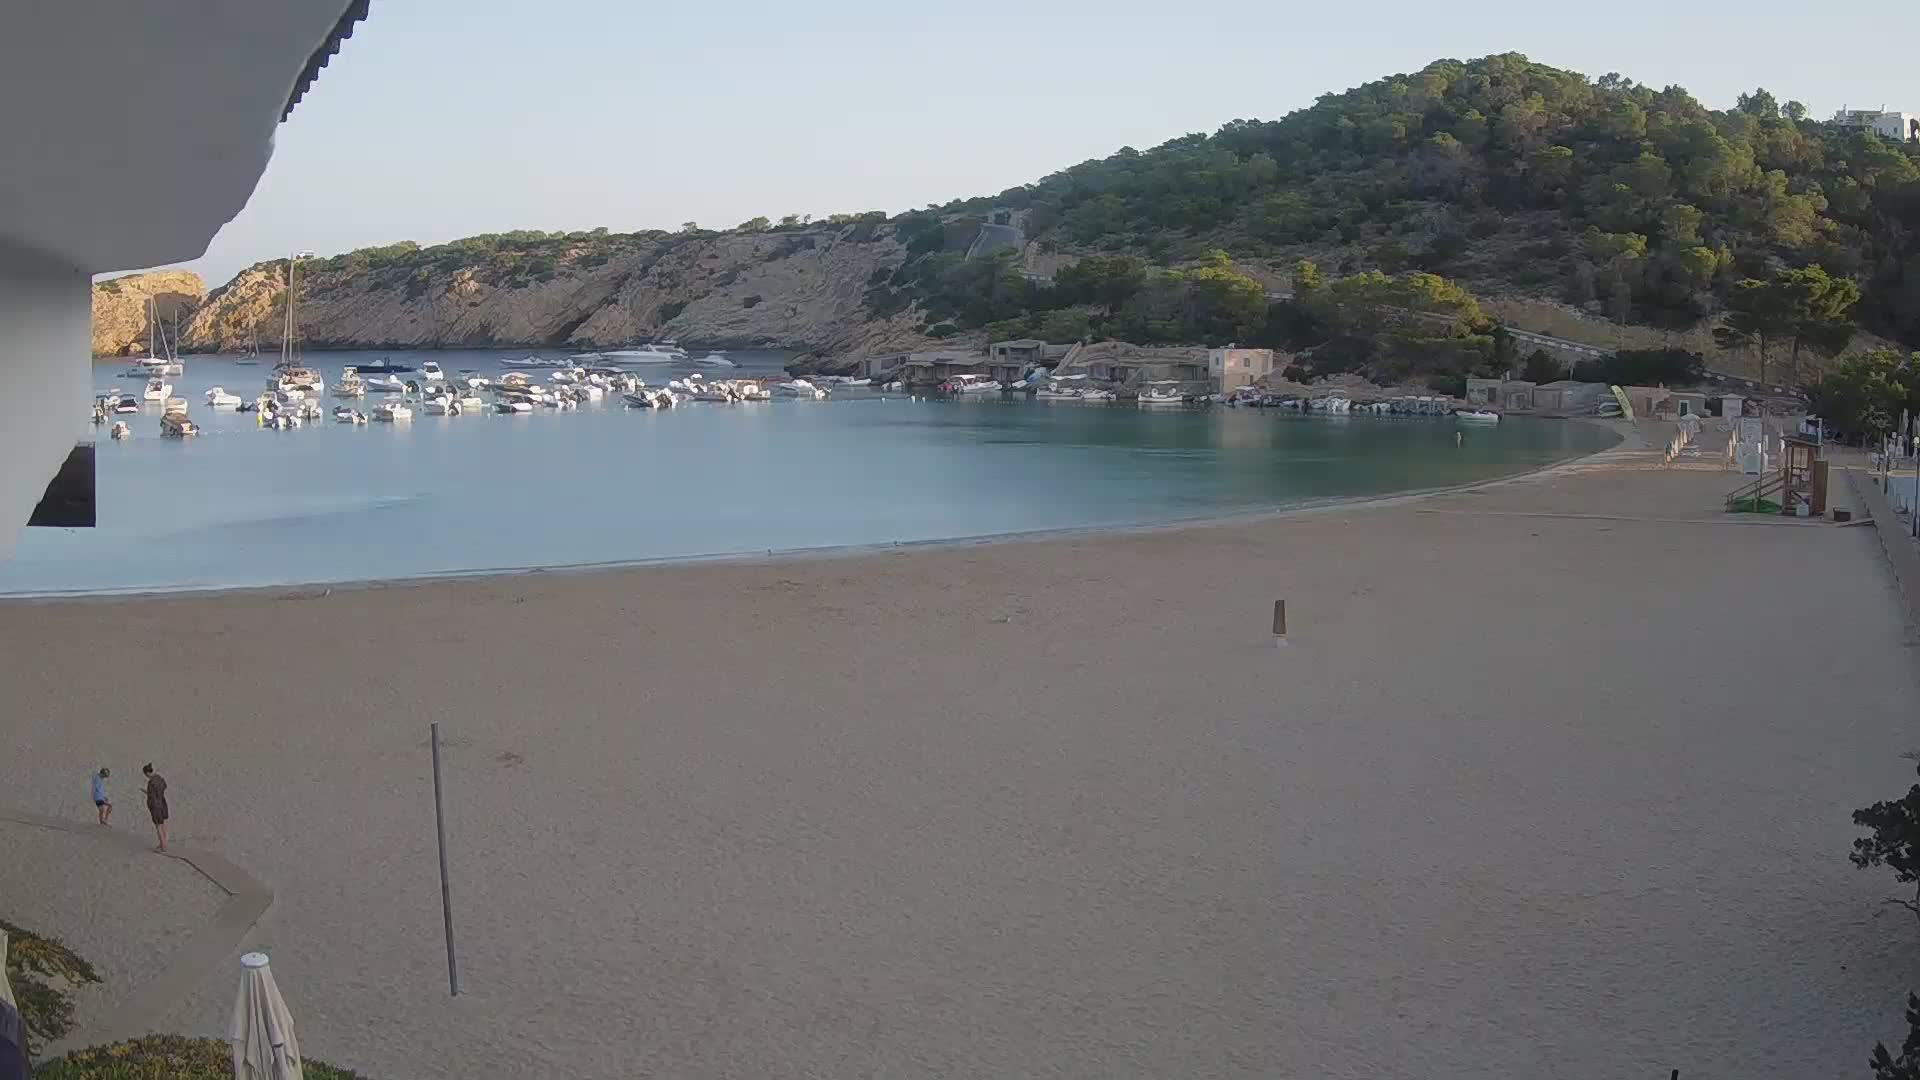
\includegraphics[width=\textwidth]{../Gelabert/1660284000.jpg}
    \end{figure}

\end{frame}

\subsection*{Gaussian Blur}
\begin{frame}
    \frametitle{Gaussian Blur}
    \begin{figure}
        \centering
        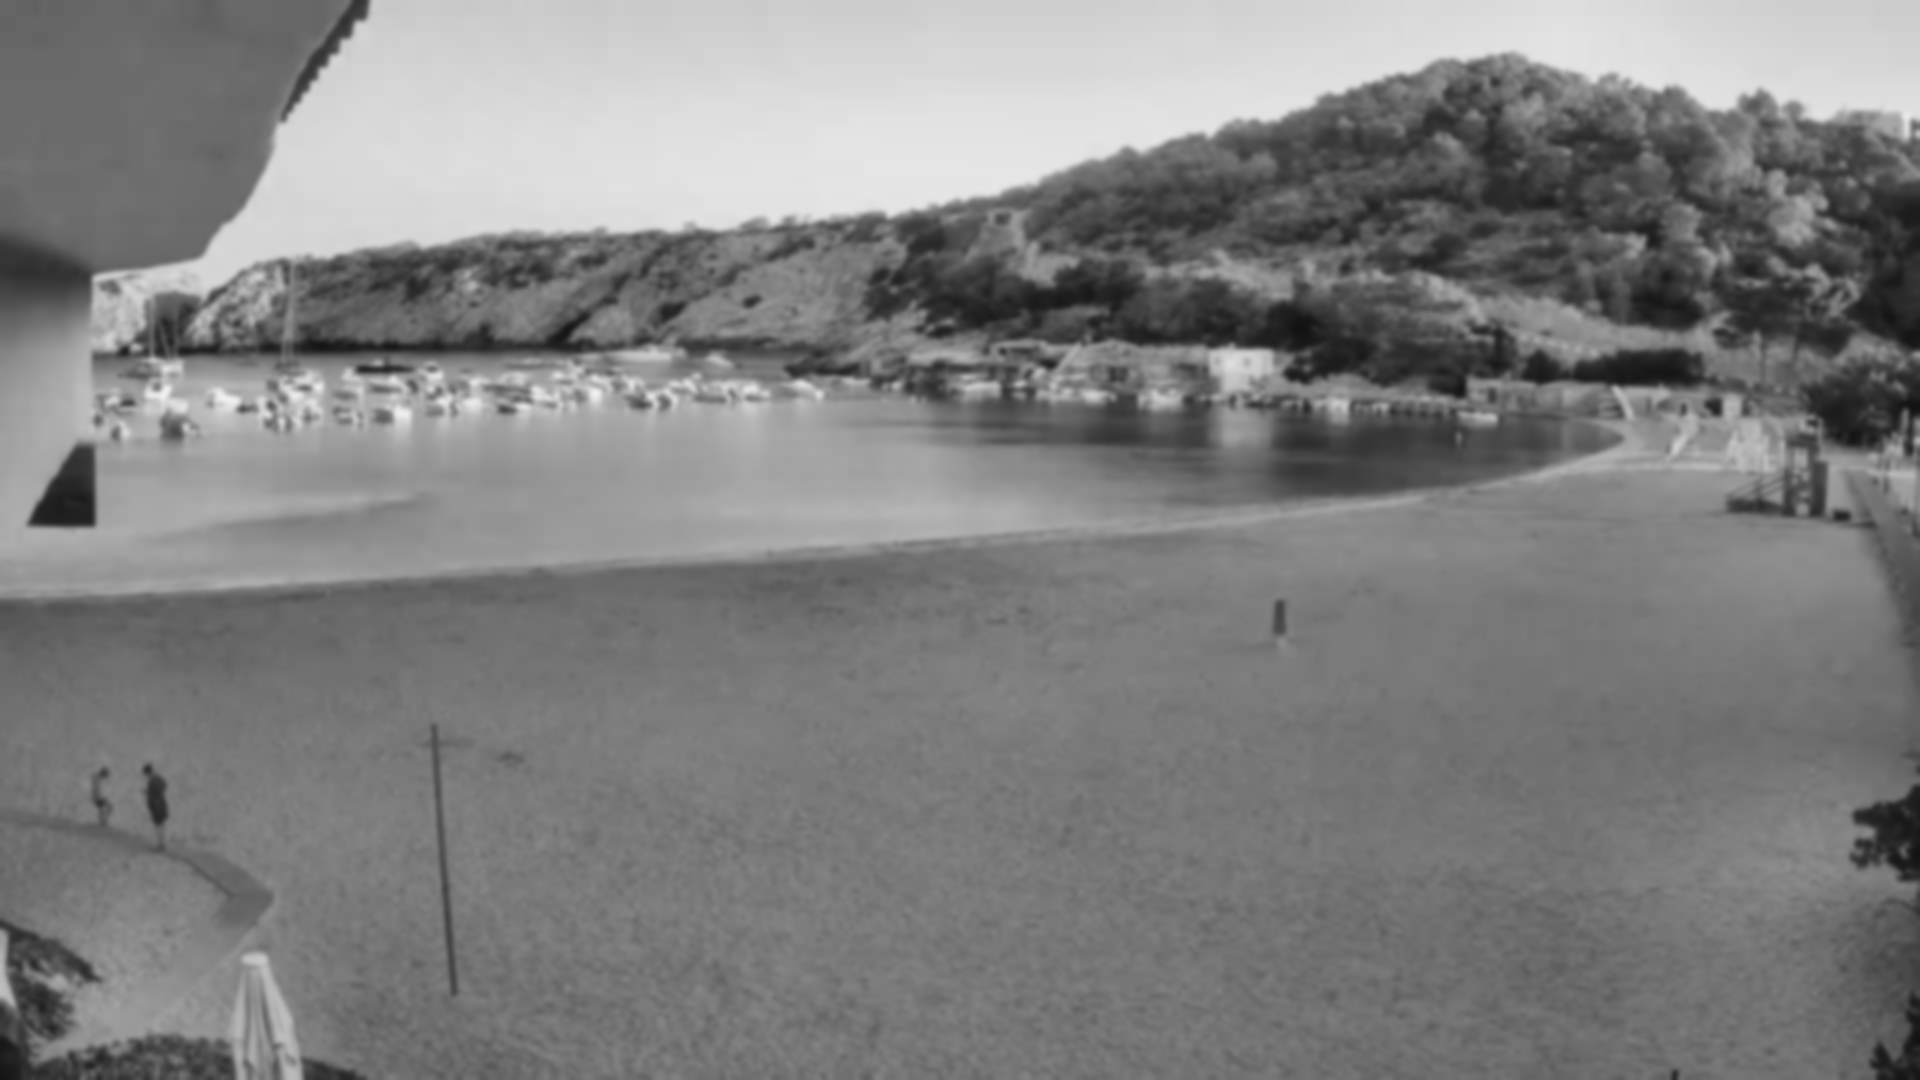
\includegraphics[width=\textwidth]{../gen/blur.png}
    \end{figure}

\end{frame}

\subsection*{Substraction}
\begin{frame}
    \frametitle{Substraction}
    \begin{figure}
        \centering
        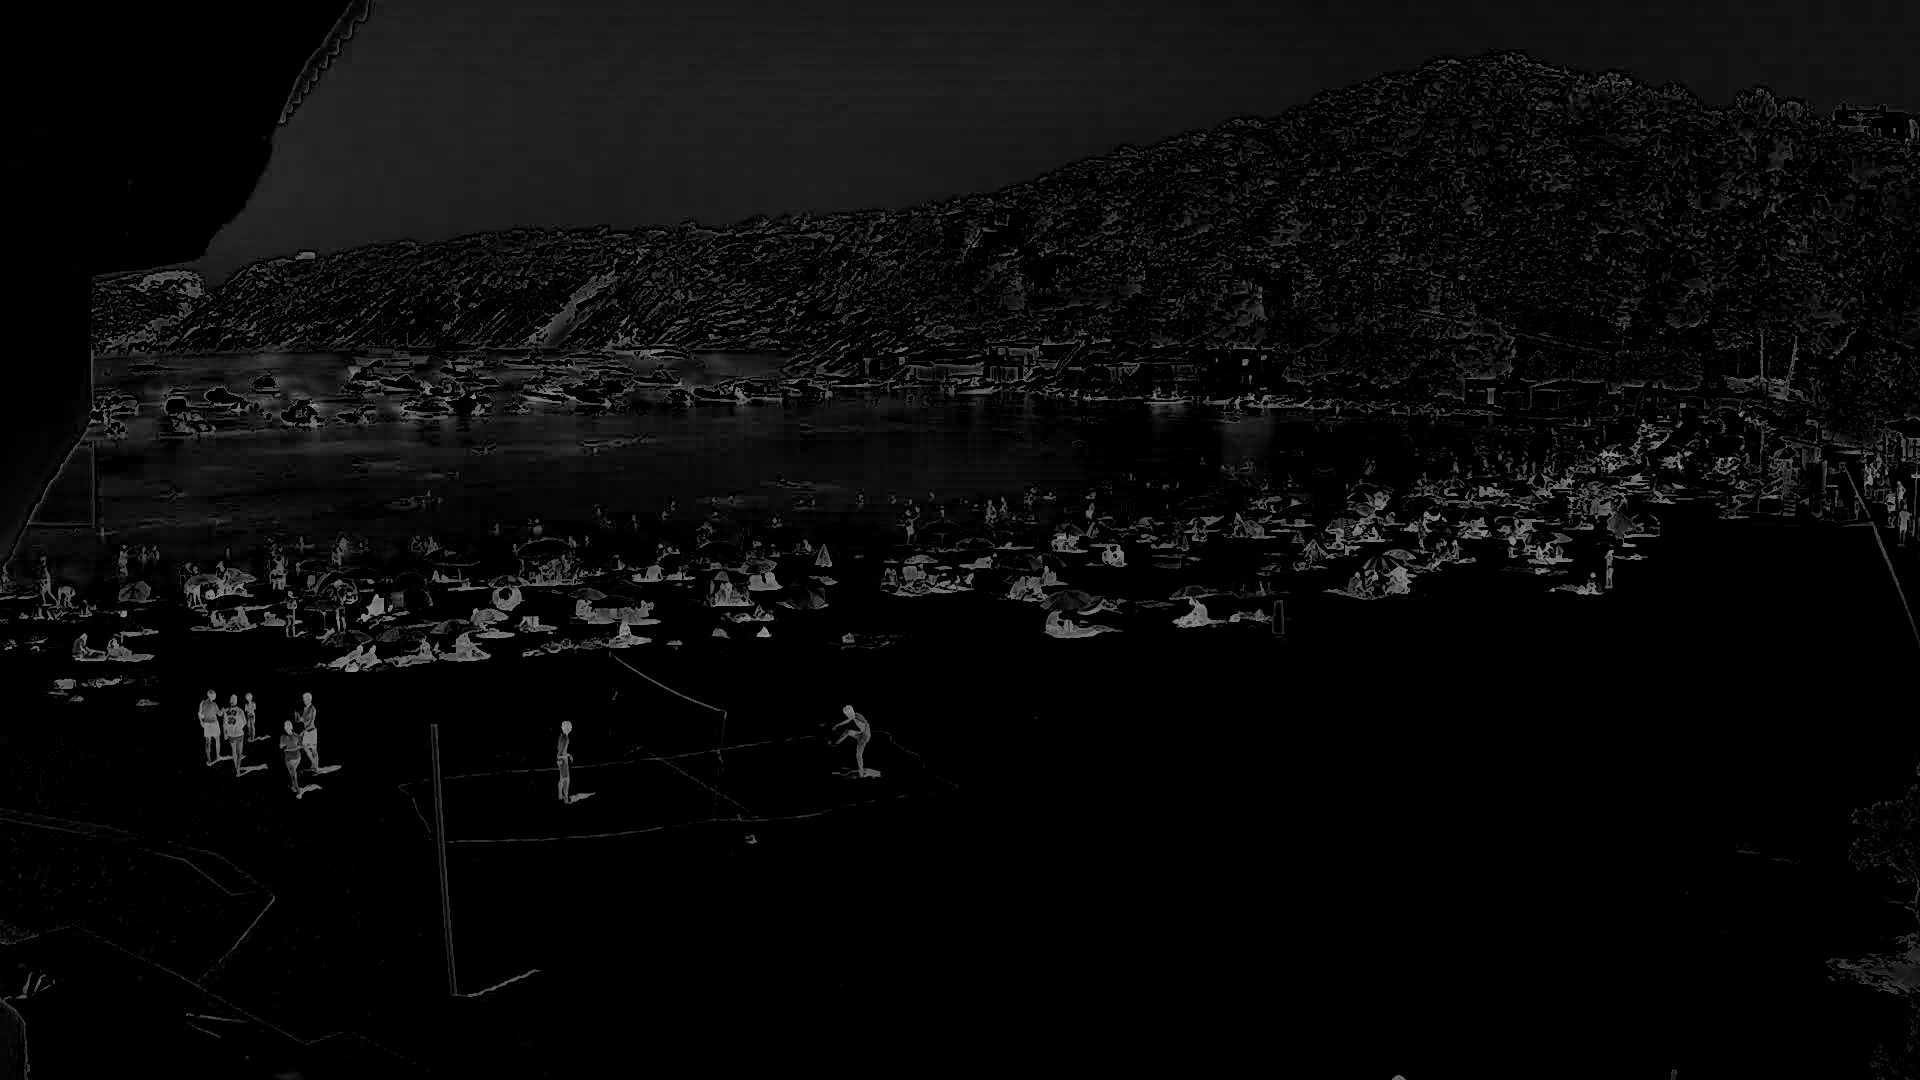
\includegraphics[width=\textwidth]{../gen/sub/1660305600.jpg}
    \end{figure}
\end{frame}

\section{Binarization}
\begin{frame}
    \frametitle{Binarization}
    \begin{figure}
        \centering
        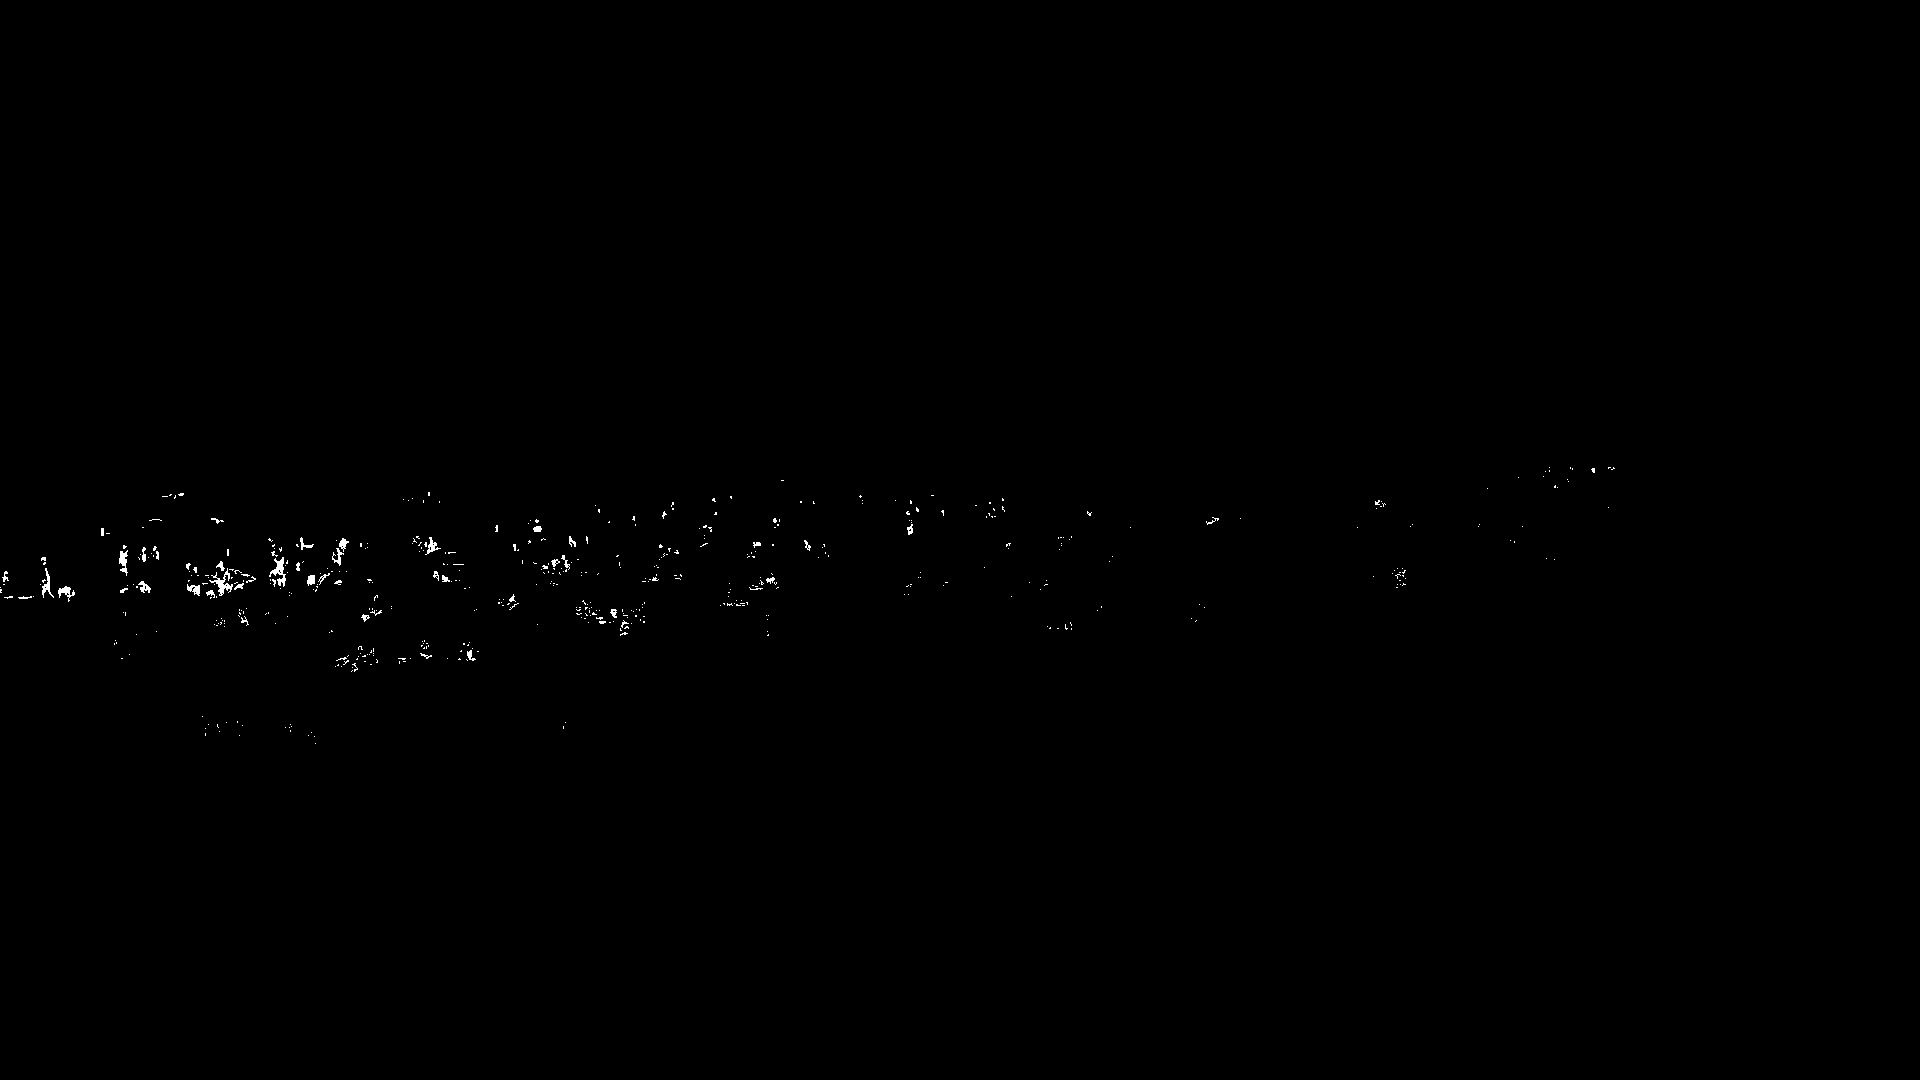
\includegraphics[width=\textwidth]{../gen/bin/1660305600.jpg}
    \end{figure}
\end{frame}

\subsection*{Masking}
\begin{frame}
    \frametitle{Masking}
    \begin{figure}
        \centering
        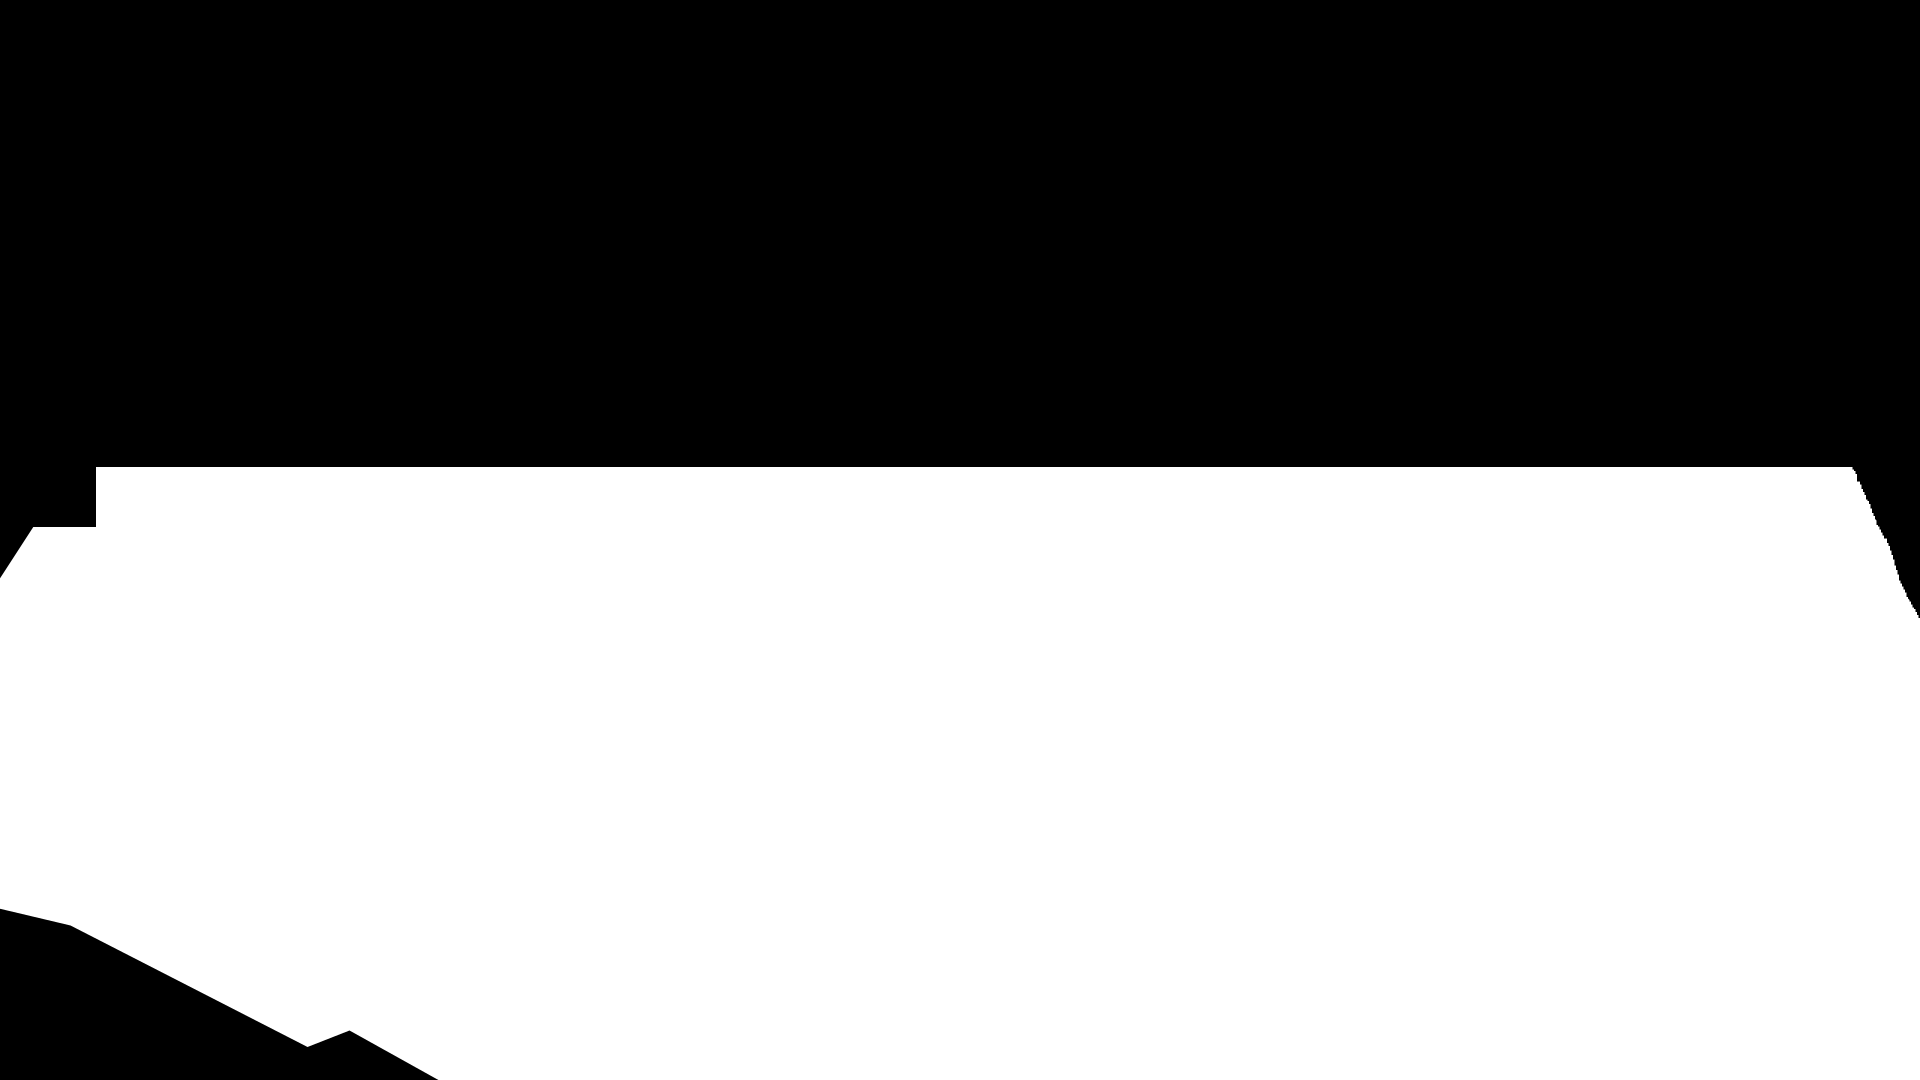
\includegraphics[width=\textwidth]{../mask.png}
    \end{figure}
\end{frame}

\section{Dilation}
\begin{frame}
    \frametitle{Dilation}

    \begin{figure}
        \centering
        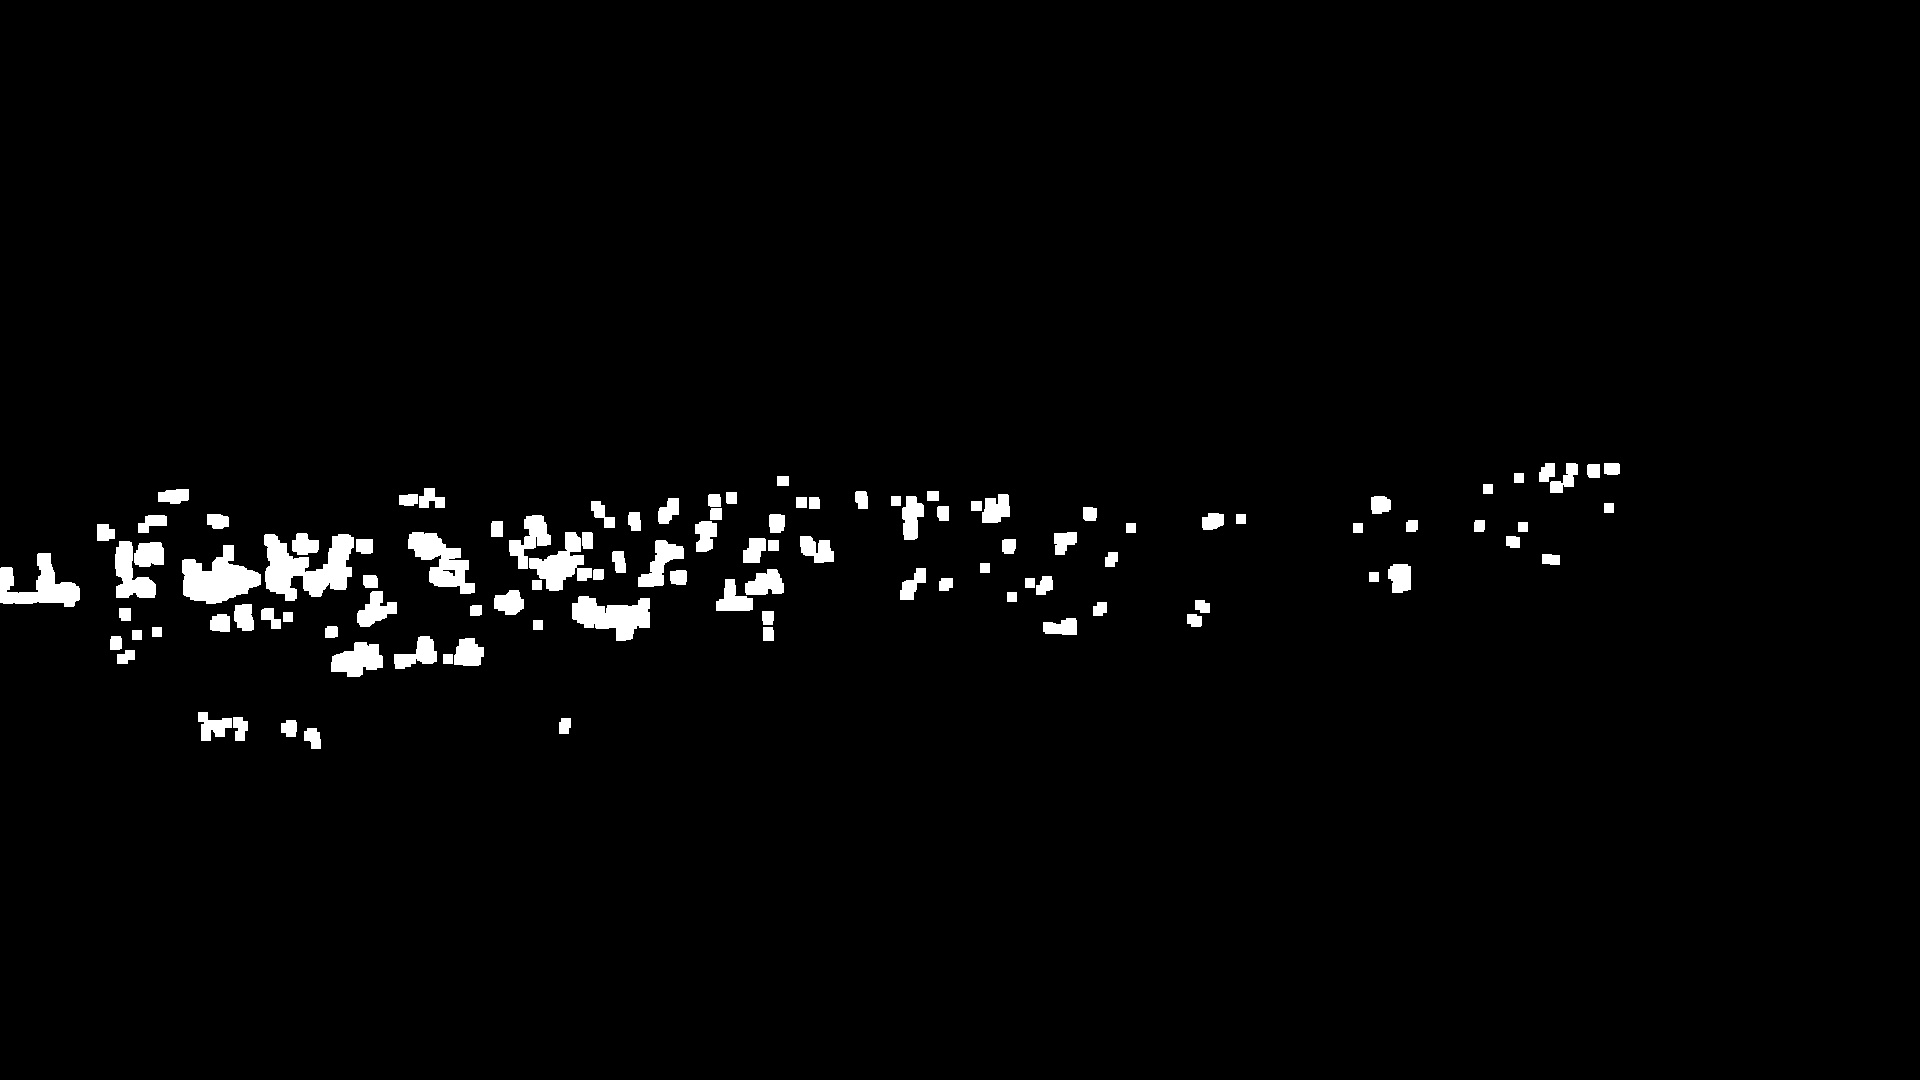
\includegraphics[width=\textwidth]{../gen/dil/1660305600.jpg}
    \end{figure}

    
\end{frame}

\section{Find contours}
\begin{frame}
    \frametitle{Find contours}
    \begin{figure}
        \centering
        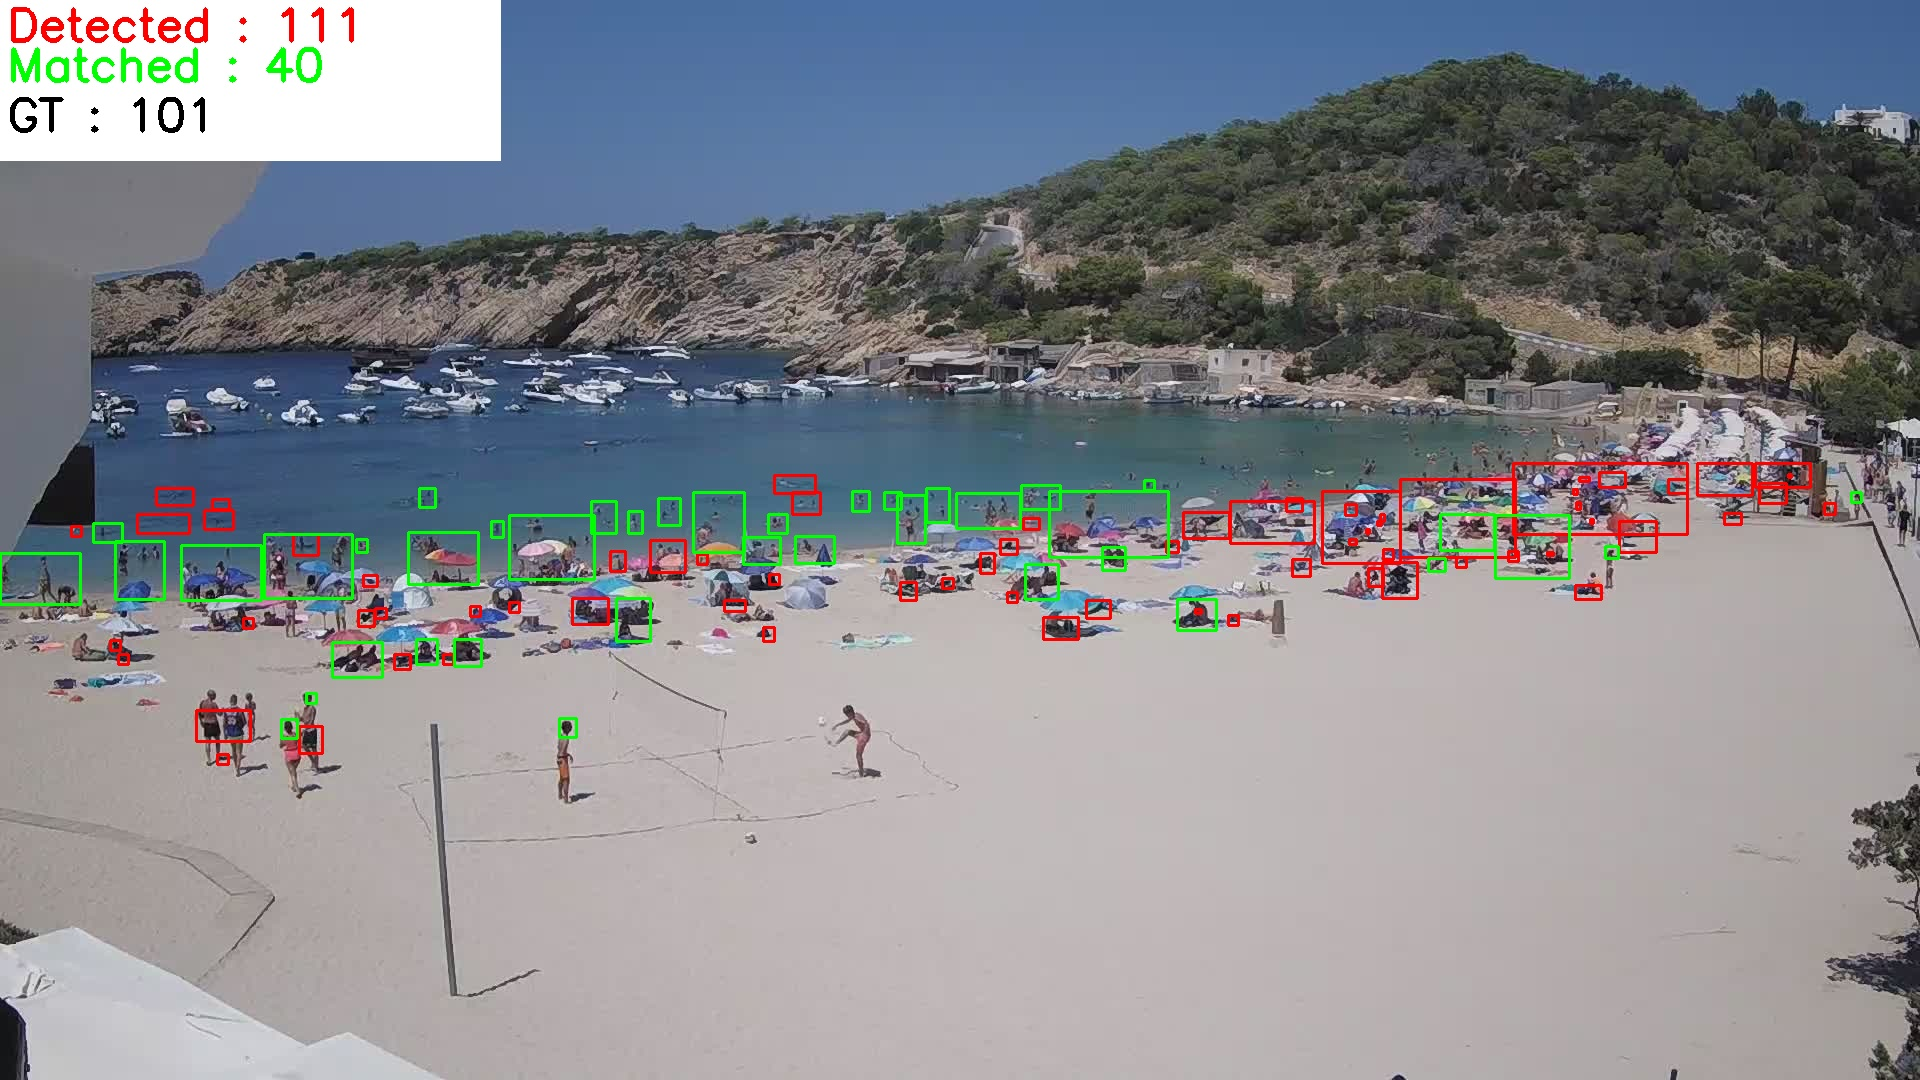
\includegraphics[width=\textwidth]{../gen/det/1660305600.jpg}
    \end{figure}
\end{frame}

\section{Real Matching}
\begin{frame}
    \frametitle{Matching}
    \begin{figure}
        \centering
        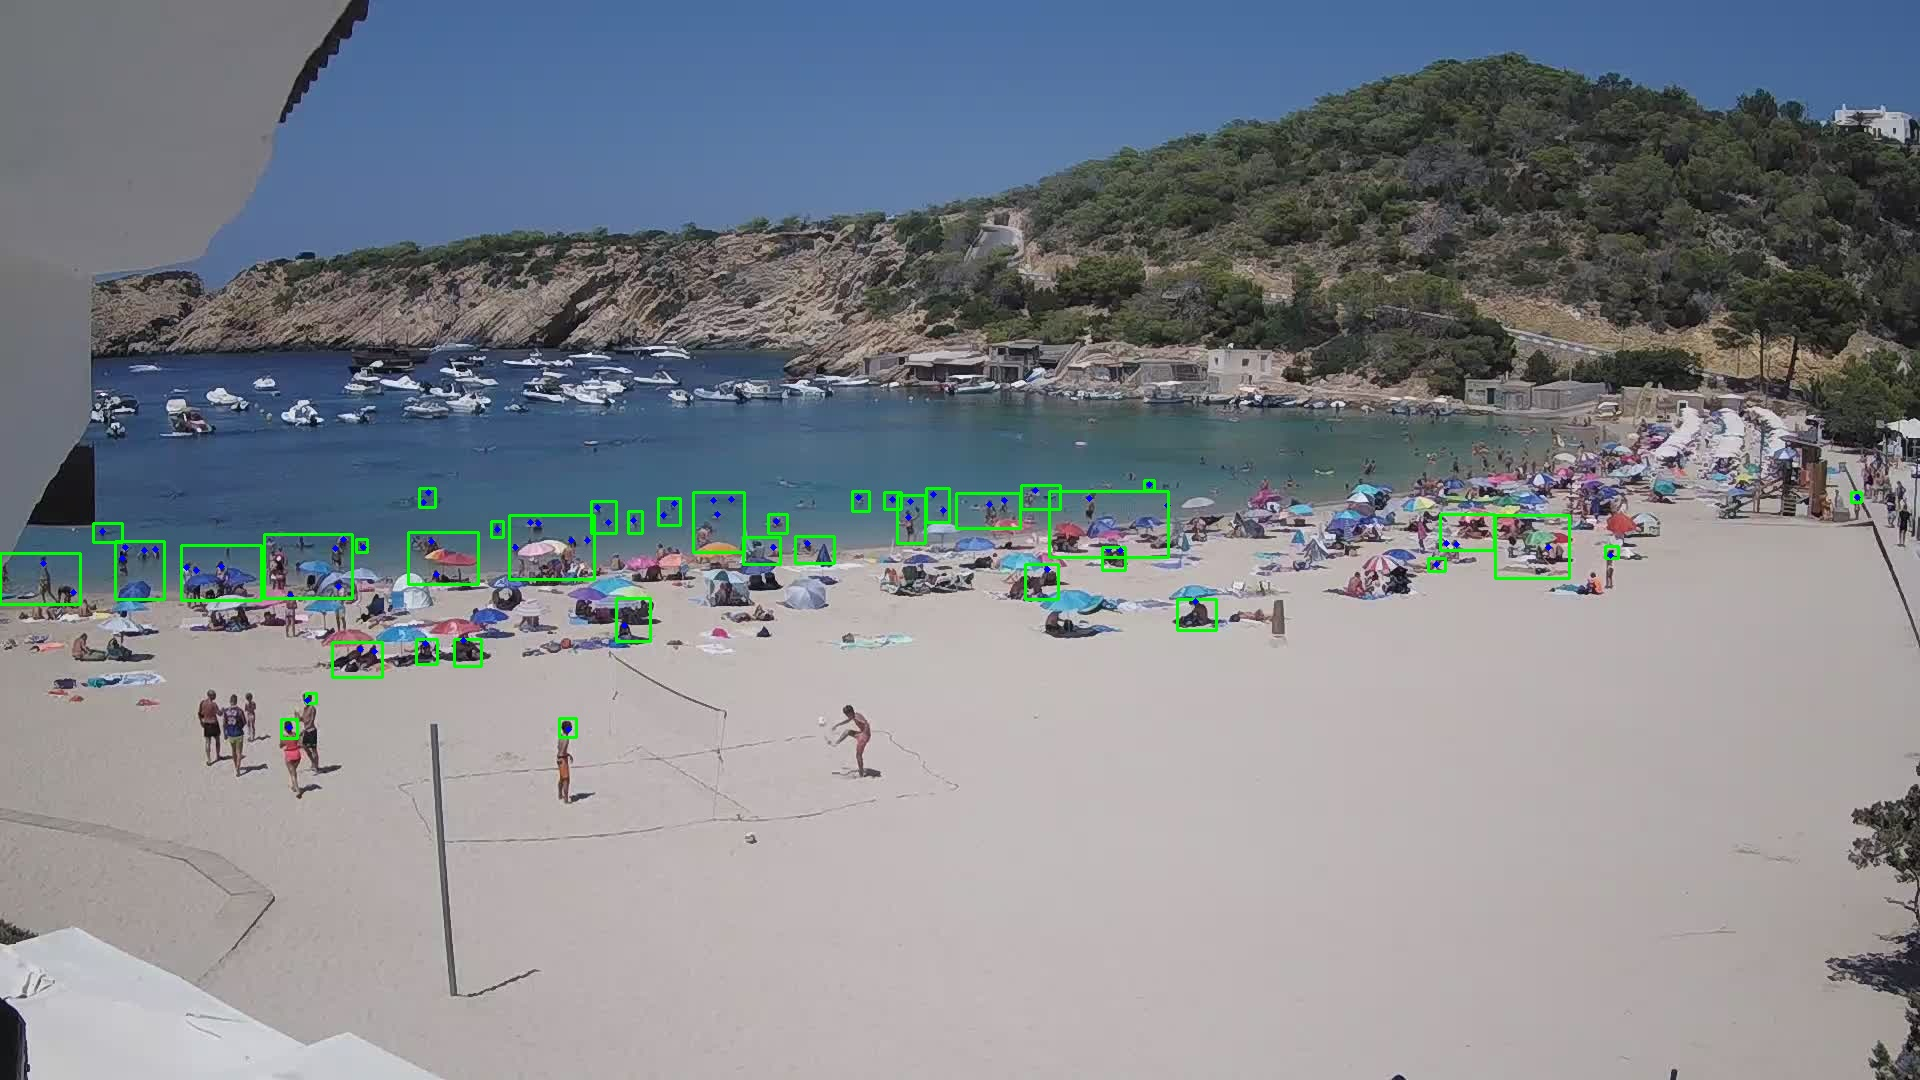
\includegraphics[width=\textwidth]{../gen/match/1660305600.jpg}
    \end{figure}
\end{frame}

\section{Conclusions}
\begin{frame}
    \frametitle{Results}

    \begin{table}
        \centering
        \caption[Performance metrics Basic]{Performance metrics using the propossed algorithm (withouth using the empty image)}\label{table:metrics}
    \csvautobooktabular{../metrics.csv}
    \end{table}

\end{frame}



\begin{frame}
    \frametitle{Conclusions}
    It is not good... but at least does something.
\end{frame}




\end{document}